\newcommand{\FigureMethodInteractPhase}{
\begin{figure}[t]
    \begin{center}
    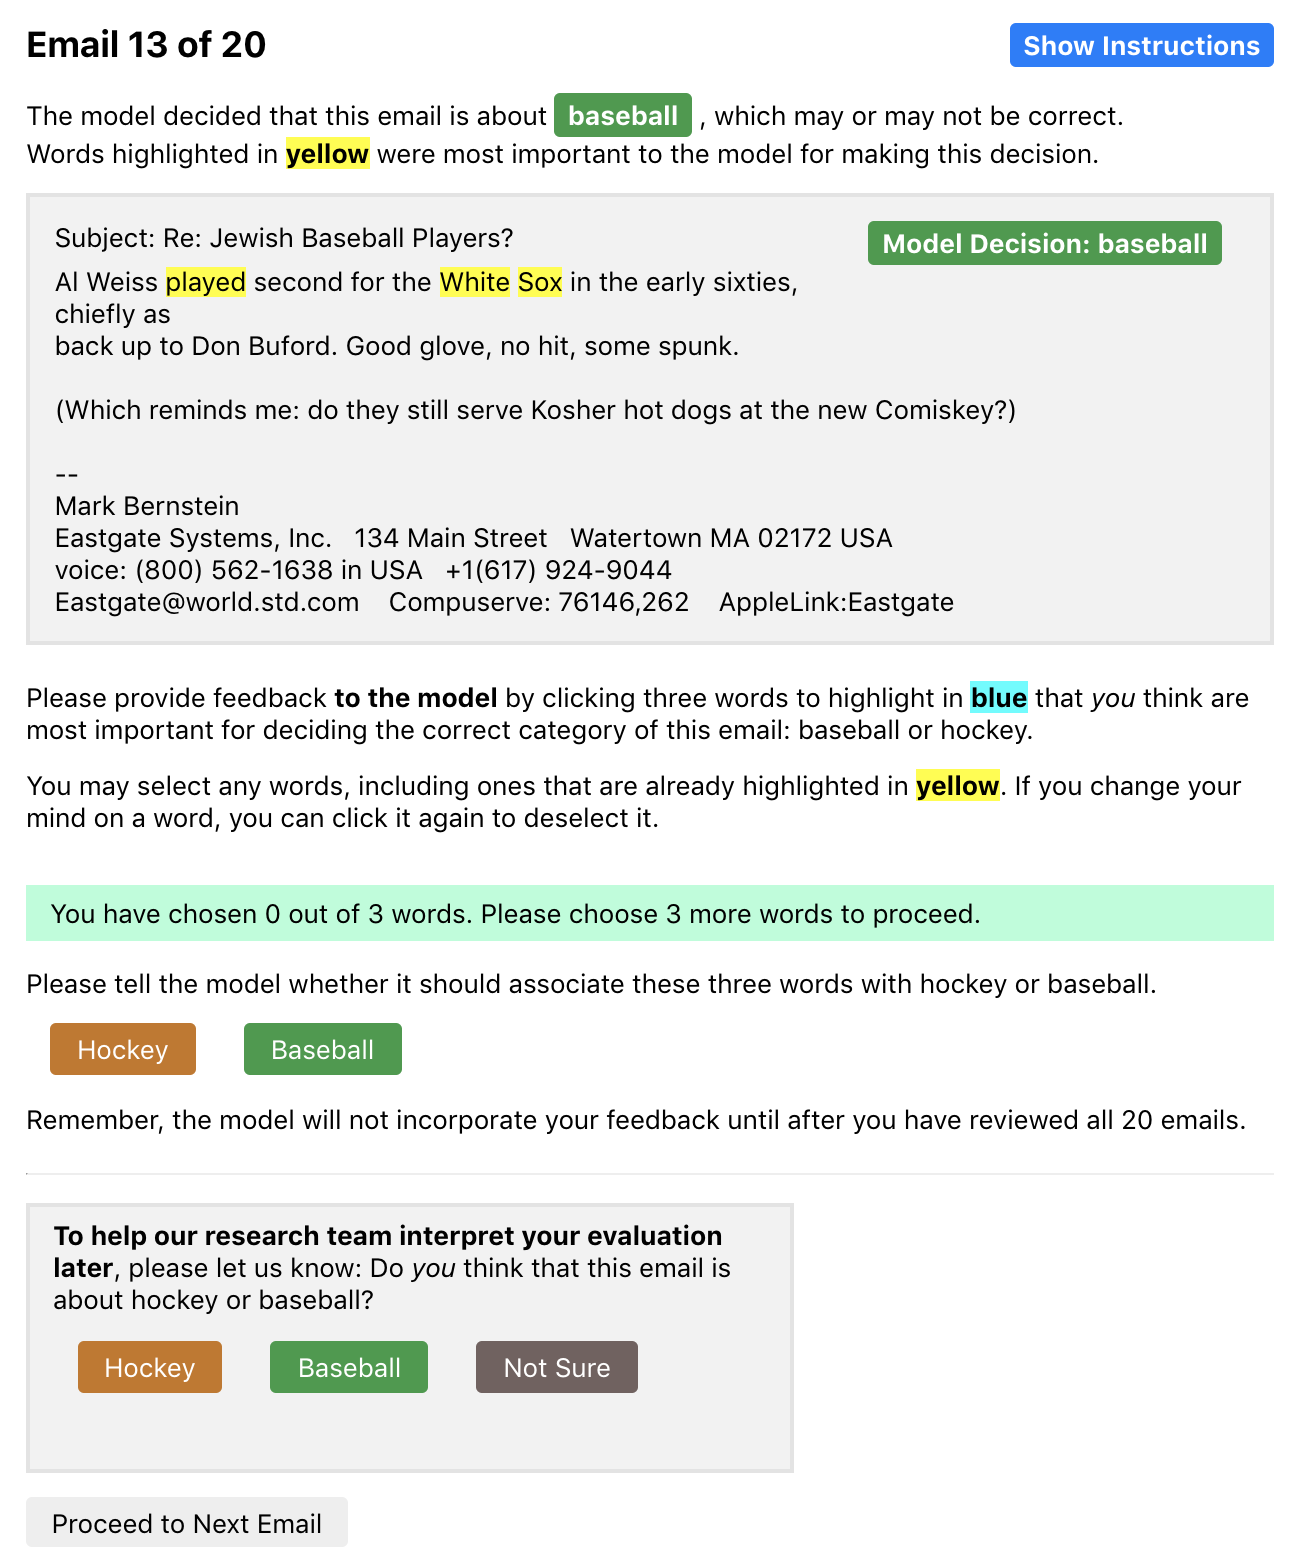
\includegraphics[width=.4\textwidth]{figures/p20_interact_email13.png}
    \end{center}
    \caption{Screenshot of an email in the ``interaction phase'' for a participant in the feature-level feedback and explanation condition (E-F).}
    \vspace{-10pt}
    \label{fig:interact_phase}
\end{figure}
}

\newcommand{\FigureMethodEvalPhase}{
\begin{figure}[t]
    \begin{center}
    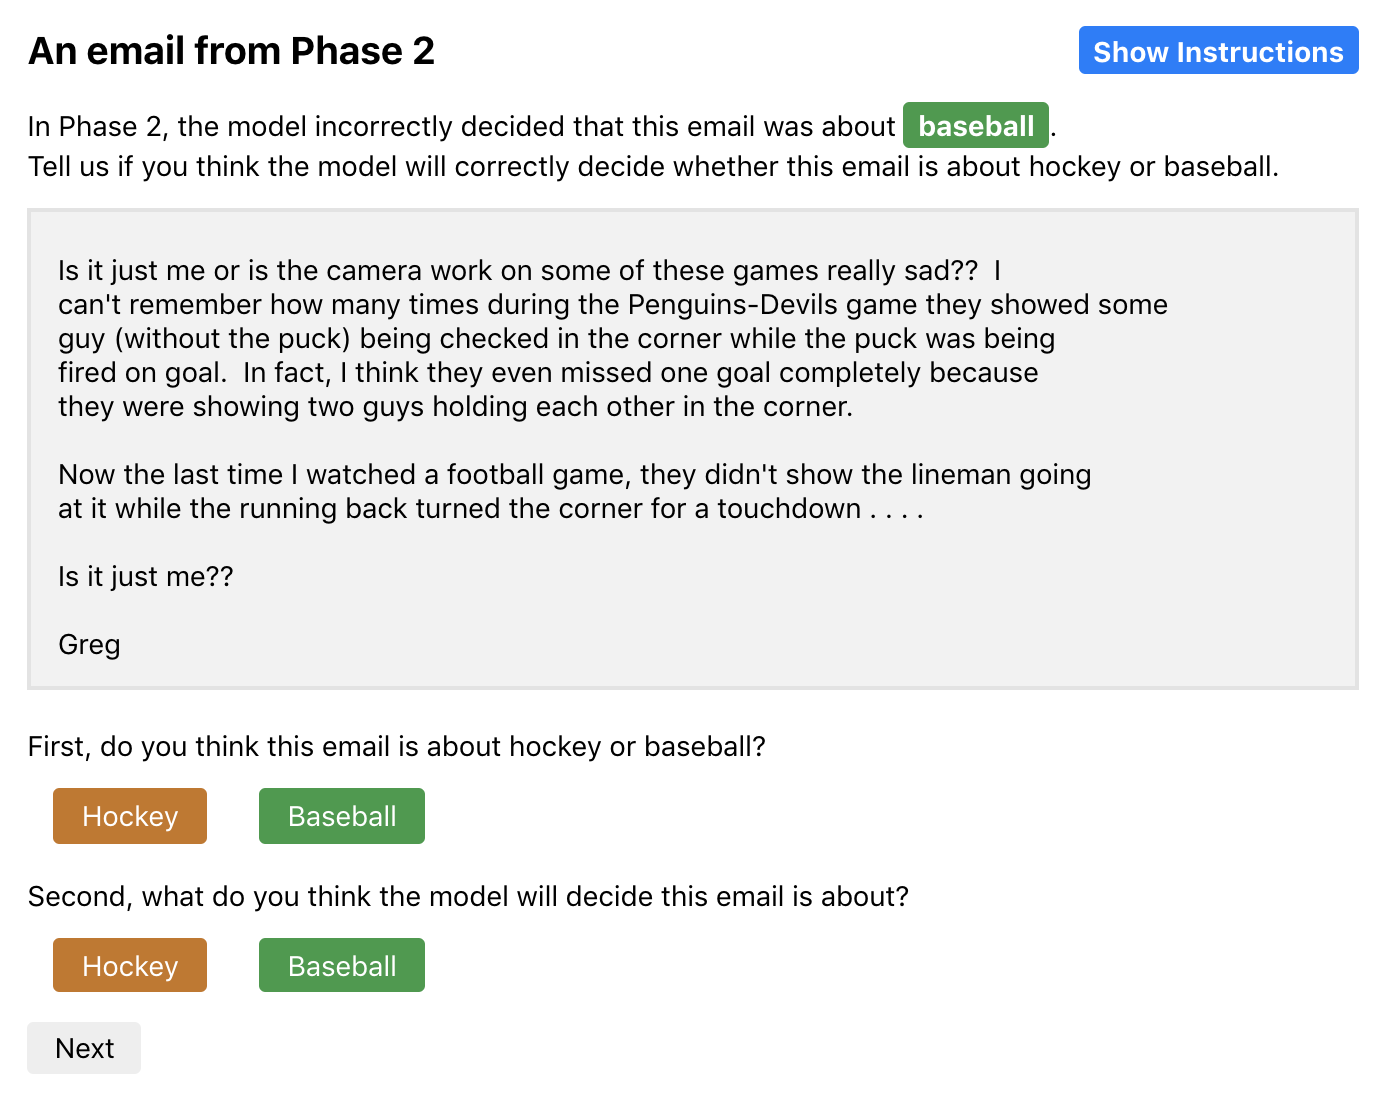
\includegraphics[width=.4\textwidth]{figures/p36_evaluate_test4.png}
    \end{center}
    \caption{Screenshot of an email in the ``evaluation phase,'' where participants predicted how the model would label an email that it had previously labeled incorrectly in the ``interaction phase.''}
    \label{fig:eval_phase}
\end{figure}
}